% Options for packages loaded elsewhere
\PassOptionsToPackage{unicode}{hyperref}
\PassOptionsToPackage{hyphens}{url}
%
\documentclass[
]{article}
\title{Plano Estratégico}
\author{Vasco Pereira}
\date{2022-02-13}

\usepackage{amsmath,amssymb}
\usepackage{lmodern}
\usepackage{iftex}
\ifPDFTeX
  \usepackage[T1]{fontenc}
  \usepackage[utf8]{inputenc}
  \usepackage{textcomp} % provide euro and other symbols
\else % if luatex or xetex
  \usepackage{unicode-math}
  \defaultfontfeatures{Scale=MatchLowercase}
  \defaultfontfeatures[\rmfamily]{Ligatures=TeX,Scale=1}
\fi
% Use upquote if available, for straight quotes in verbatim environments
\IfFileExists{upquote.sty}{\usepackage{upquote}}{}
\IfFileExists{microtype.sty}{% use microtype if available
  \usepackage[]{microtype}
  \UseMicrotypeSet[protrusion]{basicmath} % disable protrusion for tt fonts
}{}
\makeatletter
\@ifundefined{KOMAClassName}{% if non-KOMA class
  \IfFileExists{parskip.sty}{%
    \usepackage{parskip}
  }{% else
    \setlength{\parindent}{0pt}
    \setlength{\parskip}{6pt plus 2pt minus 1pt}}
}{% if KOMA class
  \KOMAoptions{parskip=half}}
\makeatother
\usepackage{xcolor}
\IfFileExists{xurl.sty}{\usepackage{xurl}}{} % add URL line breaks if available
\IfFileExists{bookmark.sty}{\usepackage{bookmark}}{\usepackage{hyperref}}
\hypersetup{
  pdftitle={Plano Estratégico},
  pdfauthor={Vasco Pereira},
  hidelinks,
  pdfcreator={LaTeX via pandoc}}
\urlstyle{same} % disable monospaced font for URLs
\usepackage[margin=1in]{geometry}
\usepackage{longtable,booktabs,array}
\usepackage{calc} % for calculating minipage widths
% Correct order of tables after \paragraph or \subparagraph
\usepackage{etoolbox}
\makeatletter
\patchcmd\longtable{\par}{\if@noskipsec\mbox{}\fi\par}{}{}
\makeatother
% Allow footnotes in longtable head/foot
\IfFileExists{footnotehyper.sty}{\usepackage{footnotehyper}}{\usepackage{footnote}}
\makesavenoteenv{longtable}
\usepackage{graphicx}
\makeatletter
\def\maxwidth{\ifdim\Gin@nat@width>\linewidth\linewidth\else\Gin@nat@width\fi}
\def\maxheight{\ifdim\Gin@nat@height>\textheight\textheight\else\Gin@nat@height\fi}
\makeatother
% Scale images if necessary, so that they will not overflow the page
% margins by default, and it is still possible to overwrite the defaults
% using explicit options in \includegraphics[width, height, ...]{}
\setkeys{Gin}{width=\maxwidth,height=\maxheight,keepaspectratio}
% Set default figure placement to htbp
\makeatletter
\def\fps@figure{htbp}
\makeatother
\setlength{\emergencystretch}{3em} % prevent overfull lines
\providecommand{\tightlist}{%
  \setlength{\itemsep}{0pt}\setlength{\parskip}{0pt}}
\setcounter{secnumdepth}{-\maxdimen} % remove section numbering
\renewcommand{\linethickness}{0.05em}
\ifLuaTeX
  \usepackage{selnolig}  % disable illegal ligatures
\fi

\begin{document}
\maketitle

\hypertarget{o-que-uxe9-o-plano-estratuxe9gico}{%
\subsection{O que é o Plano
Estratégico}\label{o-que-uxe9-o-plano-estratuxe9gico}}

O Plano Estratégico (PE) é um plano a longo prazo para a implementação
de melhorias na SUS por forma a esta aumentar a sua capacidade de
sustentabilidade e longevidade face às dificuldades inerentes à evolução
social. Sendo uma coletividade nascida em 1877, a SUS já atravessou
monarquias, ditaduras, duas pandemias virais (1920 e 2020), a presença e
ausência de moradores (implicando a drástica redução de sócios
atualmente - 2022). Já se atravessaram momentos dificeis, como
derrocadas na prórpia sede, e momentos mais prósperos.

O plano completo e em mutação conforme as necessidades o implicarem pode
ser consultado na nossa drive em:
\href{https://docs.google.com/document/d/1kXc2k4UWPusVrfWMdYjRdWl646QRQDKt_nVB_pibd7g/edit?usp=sharing}{PE}.

\hypertarget{previsuxe3o-de-balanuxe7o-atuxe9-2025}{%
\subsection{Previsão de Balanço até
2025}\label{previsuxe3o-de-balanuxe7o-atuxe9-2025}}

Com o arrendamento do espaço da cave da sede da SUS, planeamento de
limpeza regular do espaço e planeamento (ainda embrionário) da cedência
do salão nobre para atividades com a comunidade em troca de um donativo
à SUS, e com o conhecimento das despesas ao longo de 2020 e 2021,
efectuámos um plano de previsão do crescimento das contas da SUS por
forma a gerir os investimentos em obras.

Para as previsões considerou-se que:

\begin{itemize}
\item
  As despesas médias de 2020/2021 seriam acrescidas de despesa de
  limpeza com valores revistos anualmente
\item
  Previsão de 2022:\\
  - Renda de Maio a Dezembro = 8x1000 = 8000€\\
  - 10000€ de renda em atraso penhorada ao antigo inquilino\\
  - 600€ limpeza da sede\\
  - Cedência do salão 44 semanas (Yoga) = 10€ x 2horas x 2vezes por
  semana x 44 = 1760€
\item
  Previsão de 2023:\\
  - Renda = 8x1250 + 4x1000 = 14000€\\
  - 660€ limpeza da sede\\
  - Cedência do salão 50 semanas (Yoga) = 12€ x 2horas x 2vezes por
  semana x 50 = 2400€
\item
  Previsão de 2024:\\
  - Renda = 4x1250 + 8x1500 = 17000€\\
  - 720€ limpeza da sede\\
  - Cedência do salão 50 semanas (Yoga) = 15€ x 2horas x 2vezes por
  semana x 50 = 3000€
\item
  Previsão de 2025:\\
  - Renda = 4x1500 + 8x1750 = 20000€\\
  - 780€ limpeza da sede\\
  - Cedência do salão 50 semanas (Yoga) = 15€ x 2horas x 2vezes por
  semana x 50 = 3000€
\end{itemize}

O balanço das contas da SUS por ano pode ser consultado no seguinte
gráfico:

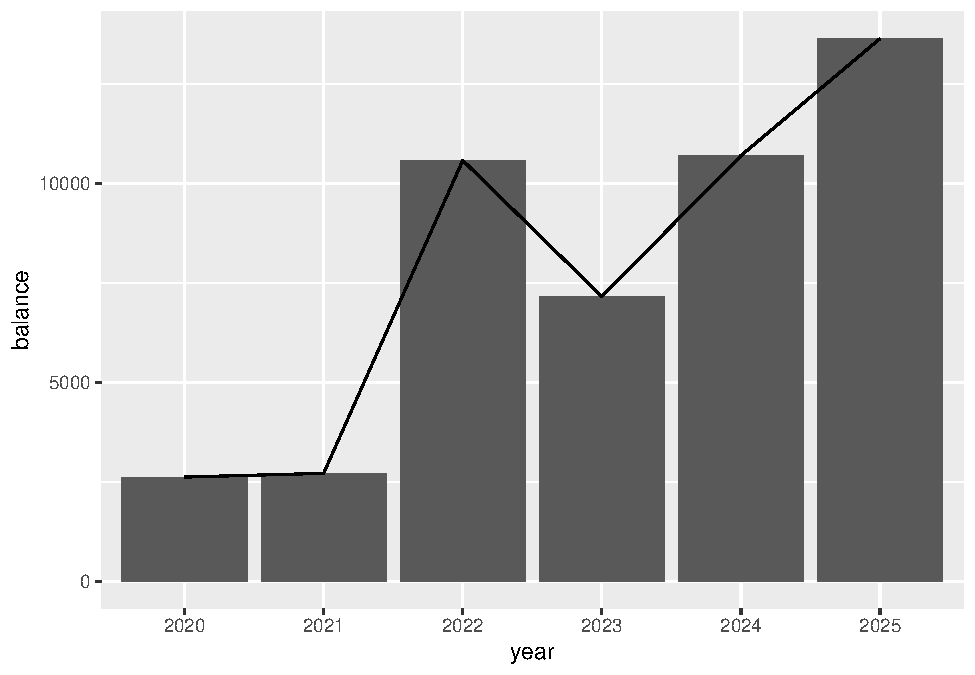
\includegraphics{PE_files/figure-latex/incomeGraph-1.pdf}

Note-se que em 2022 espera-se a entrada de rendas em atraso de 2020
ainda por serem penhoradas, pelo que isto representará um salto superior
ao esperado nesse ano.

Tabela com os balanços previstos no gráfico.

\begin{longtable}[]{@{}lr@{}}
\toprule
year & balance \\
\midrule
\endhead
2020 & 2620.460 \\
2021 & 2714.190 \\
2022 & 10575.845 \\
2023 & 7155.845 \\
2024 & 10695.845 \\
2025 & 13635.845 \\
\bottomrule
\end{longtable}

Espera-se um valor acumulado de 2023 em diante de 42063.38€. Este pode
ser investido mediante as prioridades estabelecidas no plano de
desenvolvimento.

O presente relatório é preditivo e irá mudar à medida que mais dados se
obtenham com contratos de utilização do espaço e com novos relatórios de
contas anuais.

\end{document}
